% 非互換なパッケージに自動でパッチを当てる
% https://qiita.com/wtsnjp/items/76557b1598445a1fc9da
\RequirePackage{plautopatch}
% pdfpagesの依存パッケージのエラー回避
% https://okumuralab.org/tex/mod/forum/discuss.php?d=2956
% https://github.com/aminophen/gentombow/issues/9
\plautopatchdisable{eso-pic}
% documentclassでdvipdfmx指定をするので個別パッケージでのドライバ指定は不要
% https://qiita.com/Aruneko/items/13e015bce0112143f277
\documentclass[autodetect-engine, dvi=dvipdfmx, 10pt, a4paper, ja=standard]{bxjsarticle}

% 印刷時の用紙サイズ設定
\usepackage{bxpapersize}% これでOK!

% pdf-version
\usepackage[1.4]{bxpdfver}

% 日本語環境での字体修正
\usepackage{otf}
% フォントエンコーディングの名前をオプションで指定する
\usepackage[T1]{fontenc}
\usepackage{lmodern}% Latin Modern フォントを使う

% graphicx
\usepackage{graphicx}
\usepackage{grffile}% include graphicsの画像ファイル名の制限を撤廃

% \begin{comment} ... \end{comment} で複数行コメントアウト
\usepackage{comment}

% 数学系 インライン数式を \[ \] と書く癖をつける
\usepackage{amsmath,amssymb,amsthm}
\usepackage{amsfonts}
\usepackage{mathtools}
\usepackage{bm} % bold math

% 化学
\usepackage[version=4]{mhchem}

% SI単位系
\usepackage{siunitx}

% 表関連
\usepackage{multirow} % 表のセルの結合
\usepackage{booktabs} % 表の線がすごくなる. Table Generatorを使うときはbooktabsモードにする
\usepackage{caption} % キャプションをいじる
\usepackage{float} % 図表を絶対にそこに置く確固たる意思

% その他便利な子
\usepackage{pdfpages} % pdfを挿入
\usepackage[hyphens]{url} % urlをきれいに表示する
\usepackage{ulem} % 下線を強化
\usepackage[at]{easylist} % @をつかって箇条書き
% \usepackage{minted}
% \usepackage{termsim} % ターミナルを再現...誰得?

% ハイパーリンクを生成
% sectionなどで数式を使う場合は \texorpdfstring{texstring}{pdfstring}をする
\usepackage{hyperref}
\usepackage{pxjahyper}
\usepackage{footnotebackref} % 脚注から本文へ飛べる


% ここからはソースコードを表示する設定
\usepackage{listings, plistings, color}
\renewcommand{\lstlistingname}{Code}
\definecolor{OliveGreen}{rgb}{0.0,0.6,0.0}
\definecolor{Orenge}{rgb}{0.89,0.55,0}
\definecolor{SkyBlue}{rgb}{0.28, 0.28, 0.95}
\lstset{
    language={Ruby}, % 言語の指定
    basicstyle={\ttfamily},
    identifierstyle={\small},
    commentstyle={\smallitshape},
    keywordstyle={\small\bfseries},
    ndkeywordstyle={\small},
    stringstyle={\small\ttfamily},
    frame={tb},
    breaklines=true,
    columns=[l]{fullflexible},
    numbers=left,
    xrightmargin=0zw,
    xleftmargin=3zw,
    numberstyle={\scriptsize},
    stepnumber=1,
    numbersep=1zw,
    lineskip=-0.5ex,
    stepnumber=1,       % 行数の増間
    numbersep=1zw,      % 行数の余白
    xrightmargin=0zw,   % 左の余白
    xleftmargin=2zw,    % 右の余白
    framexleftmargin=18pt,  % フレームからの左の余白
    keepspaces=true,    % スペースを省略せず保持
    lineskip=-0.2ex,    % 枠線の途切れ防止
    tabsize = 4,        % タブ数
    showstringspaces=false,  %文字列中の半角スペースを表示させない
    keywordstyle={\color{SkyBlue}},     %キーワード(int, ifなど)の書体指定
    commentstyle={\color{OliveGreen}},  %注釈の書体
    stringstyle=\color{Orenge}          %文字列
}

% \refだけで「図」や「式」を自動挿入
% https://zenn.dev/arks/articles/3697b25d03f8a8
% subfigureが文書にあると小節を参照する際に使う\subrefがおかしくなるので注意
%% increase link area for cross-references and autoname them, [130514]
\AtBeginDocument{\renewcommand{\ref}[1]{\mbox{\autoref{#1}}}}

\def\equationautorefname~#1\null{式(#1)\null}
\def\figureautorefname~#1\null{図#1\null}
\def\subfigureautorefname#1\null{図#1\null}
\def\tableautorefname~#1{表#1}
\def\lstlistingautorefname~#1{コード#1}

\def\partautorefname#1\null{第#1部\null}
\def\chapterautorefname#1\null{第#1章\null}
\def\sectionautorefname#1\null{#1節}
\def\subsectionautorefname~#1\null{#1節}
\def\subsubsectionautorefname#1\null{#1節}
\def\paragraphautorefname#1\null{#1段落}
\def\subparagraphautorefname#1\null{#1段落}

\def\Itemautorefname#1\null{項目#1\null}
\def\Hfootnoteautorefname#1\null{脚注#1\null}
\def\theoremautorefname#1\null{定理#1\null}
\def\FancyVerbLineautorefname#1\null{#1行\null}
% \def\pageautorefname#1\null{ページ#1\null}
\def\appendixautorefname#1\null{付録#1\null}


\title{MICS実験第一 J4課題レポート}
\author{学籍番号 2210342, 鈴木謙太郎}
\date{\today}
\begin{document}
\maketitle


\section{課題1}
\label{sec:ex-1}

まず,writeシステムコールを直接用いる\ref{code:ex-1}のようなmycp関数を作成した.

\begin{lstlisting}[language={C}, caption={mycp関数のソースコード}, label={code:ex-1}]
#include <fcntl.h>
#include <stdio.h>
#include <stdlib.h>
#include <unistd.h>

#define BUFFER_SIZE 128

void mycp(const char *src, const char *dst, size_t buffer_size) {
  int src_fd = open(src, O_RDONLY);
  if (src_fd == -1) {
    perror("Error opening source file");
    exit(EXIT_FAILURE);
  }

  int dst_fd = open(dst, O_WRONLY | O_CREAT | O_TRUNC, 0644);
  if (dst_fd == -1) {
    perror("Error opening destination file");
    close(src_fd);
    exit(EXIT_FAILURE);
  }

  char *buffer = (char *)malloc(buffer_size);
  if (buffer == NULL) {
    perror("Error allocating buffer");
    close(src_fd);
    close(dst_fd);
    exit(EXIT_FAILURE);
  }

  ssize_t bytes_read;
  while ((bytes_read = read(src_fd, buffer, buffer_size)) > 0) {
    if (write(dst_fd, buffer, bytes_read) != bytes_read) {
      perror("Error writing to destination file");
      free(buffer);
      close(src_fd);
      close(dst_fd);
      exit(EXIT_FAILURE);
    }
  }

  if (bytes_read == -1) {
    perror("Error reading from source file");
  }

  free(buffer);
  close(src_fd);
  close(dst_fd);
}

int main(int argc, char const *argv[]) {
  if (argc != 3) {
    fprintf(stderr, "Usage: %s <source> <destination>\n", argv[0]);
    return 1;
  }
  char const *source = argv[1];
  char const *destination = argv[2];
  mycp(source, destination, BUFFER_SIZE);
  return 0;
}

\end{lstlisting}

また,このmycp関数の性能を評価する際の対照として,\ref{code:ex-2}のような標準ライブラリ関数を用いたコピー関数を作成した.

\begin{lstlisting}[language={C}, caption={比較用のコピー関数のソースコード}, label={code:ex-2}]
#include <stdio.h>
#include <stdlib.h>

void copy_file_stdio(const char *src, const char *dst) {
  FILE *src_file = fopen(src, "rb");
  if (src_file == NULL) {
    perror("Error opening source file");
    exit(EXIT_FAILURE);
  }

  FILE *dst_file = fopen(dst, "wb");
  if (dst_file == NULL) {
    perror("Error opening destination file");
    fclose(src_file);
    exit(EXIT_FAILURE);
  }

  int ch;
  while ((ch = fgetc(src_file)) != EOF) {
    if (fputc(ch, dst_file) == EOF) {
      perror("Error writing to destination file");
      fclose(src_file);
      fclose(dst_file);
      exit(EXIT_FAILURE);
    }
  }

  fclose(src_file);
  fclose(dst_file);
}

int main(int argc, char const *argv[]) {
  if (argc != 3) {
    fprintf(stderr, "Usage: %s <source> <destination>\n", argv[0]);
    return 1;
  }
  char const *source = argv[1];
  char const *destination = argv[2];
  copy_file_stdio(source, destination);
  return 0;
}

\end{lstlisting}

これらの関数を用いて,コピー対象とするファイルのサイズを$16^1 \sim 16^9$バイトの間で変えながら,それぞれの関数の性能を評価した.
性能評価には,GNU timeコマンドを用い,実行時間を$10^{-2}$秒単位で測定した.

まず,mycp関数の測定結果は\ref{fig:ex-1-mycp}のようになった.

\begin{figure}[H]
	\centering
	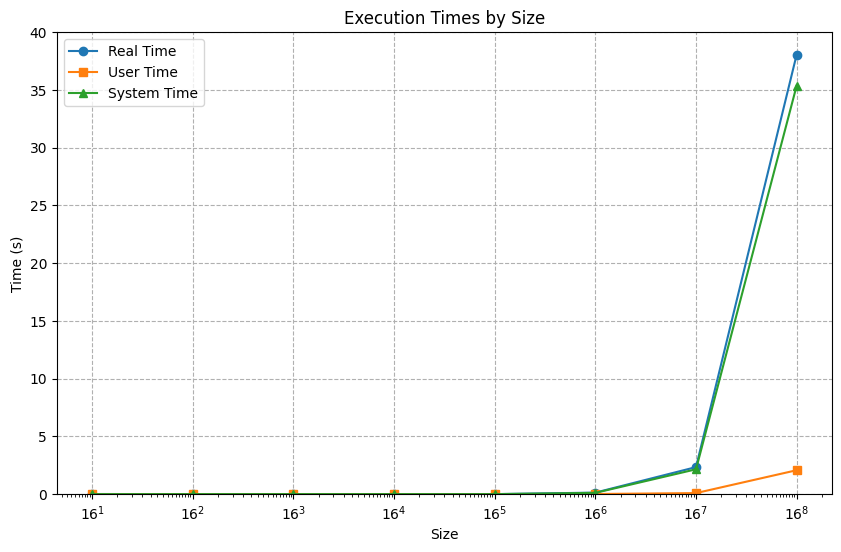
\includegraphics[width=0.8\linewidth]{./mycp.png}
	\caption{mycp関数の性能測定結果}
	\label{fig:ex-1-mycp}
\end{figure}

次に,標準ライブラリ関数を用いたコピー関数の測定結果は\ref{fig:ex-1-stdio}のようになった.

\begin{figure}[H]
	\centering
	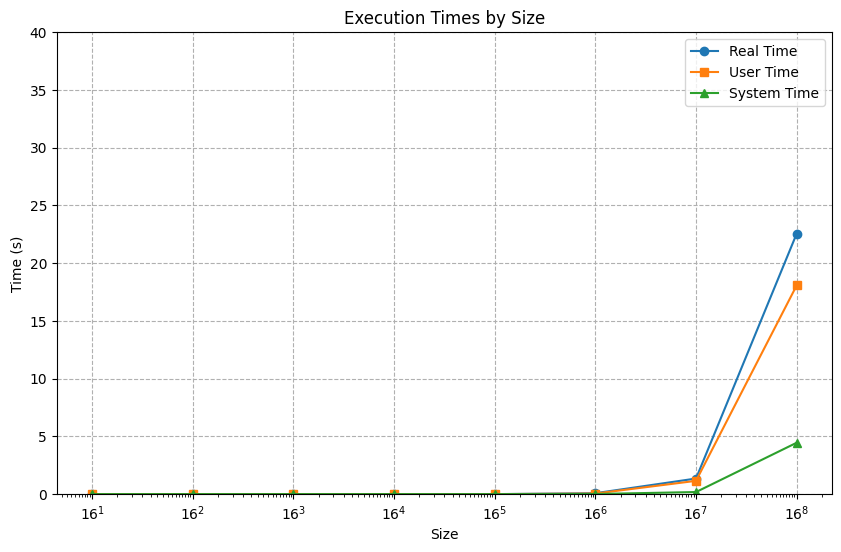
\includegraphics[width=0.8\linewidth]{./syscp.png}
	\caption{標準ライブラリ関数を用いたコピー関数の性能測定結果}
	\label{fig:ex-1-stdio}
\end{figure}

2つの関数の測定結果で共通している点は,ファイルサイズが$16^6$バイト($1$メガバイト)程度までは$10^{-2}$秒単位での実行時間がほぼ一定であることである.
また,ファイルサイズが$16^7$バイト($10$メガバイト)程度を超えると,どちらの関数も実行時間がtimeコマンドで測定できる程度になることがわかる.

一方で,実行時間が増えてきてからの傾向については,mycp関数と標準ライブラリ関数を用いたコピー関数で異なる点がみられる.
独自に作成したmycp関数の実行時間はsystem timeが占める割合が大きいが,標準ライブラリ関数を用いたコピー関数の実行時間はuser timeが占める割合が大きい.

この違いとしては, システムコールの回数の違いが考えられる.
mycp関数は,readとwriteのシステムコールを用いてファイルのコピーを行っているため,システムコールの回数が多くなる.
一方で,標準ライブラリ関数を用いたコピー関数は,ファイルの読み書きを行う際にバッファリングを行っているため,システムコールの回数が少なくなる.
fgetc/fputcは1バイトずつ読み取りと書き込みを行っているが,内部的にはある程度大きなバッファで読み書きを行っているため,システムコールの回数が少なくなっていると推測される.

このような結果,システムコールの回数が異なっているので,2つの関数において実行時間の内訳が異なると考えられる.

\section{課題2}
\label{sec:ex-2}

可変長引数としてホスト名を複数渡すと,それらに対してpingを実行する関数を作成する.

まず,指定されたホストに対して並行でpingを実行する関数を\ref{code:ex-2-parallel}のように作成した.

\begin{lstlisting}[language={C}, caption={pingを並行して実行する関数}, label={code:ex-2-parallel}]
#include <stdio.h>
#include <stdlib.h>
#include <sys/wait.h>
#include <unistd.h>

int main(int argc, char *argv[]) {
  if (argc < 2) {
    fprintf(stderr, "Usage: %s host1 host2 ...\n", argv[0]);
    return 1;
  }

  for (int i = 1; i < argc; ++i) {
    pid_t pid = fork();

    if (pid == -1) {
      // フォーク失敗
      perror("fork failed");
      return 1;
    } else if (pid == 0) {
      // 子プロセス
      execlp("ping", "ping", "-c", "3", argv[i], (char *)NULL);
      perror("execlp failed");
      exit(1);
    } else {
      // 親プロセス
      // 何もしない
    }
  }

  // 親プロセスは全ての子プロセスが終了するのを待つ
  for (int i = 1; i < argc; ++i) {
    wait(NULL);
  }

  return 0;
}
\end{lstlisting}

同様に,指定されたホストに対して直列にpingを実行する関数を\ref{code:ex-2-serial}のように作成した.

\begin{lstlisting}[language={C}, caption={pingを並行して実行する関数}, label={code:ex-2-serial}]
#include <stdio.h>
#include <stdlib.h>
#include <sys/wait.h>
#include <unistd.h>

int main(int argc, char const* argv[]) {
  if (argc < 2) {
    fprintf(stderr, "Usage: %s host1 host2 ...\n", argv[0]);
    return 1;
  }

  for (int i = 1; i < argc; i++) {
    pid_t pid = fork();

    if (pid == -1) {
      // フォーク失敗
      perror("fork");
      return 1;
    } else if (pid == 0) {
      // 子プロセス
      execlp("ping", "ping", "-c", "3", argv[i], (char*)NULL);
      perror("execvp");
      exit(1);
    } else {
      // 親プロセス
      int status;
      waitpid(pid, &status, 0);  // 子プロセスの終了を待つ
    }
  }

  return 0;
}
\end{lstlisting}

これらの関数に対して,9つのホスト名を指定し,実行にかかった時間をGNU timeコマンドで測定した結果は\ref{fig:ex-2}のようになった.
並行に実行した結果がparallel,直列に実行した結果がserialである.

\begin{figure}[H]
	\centering
	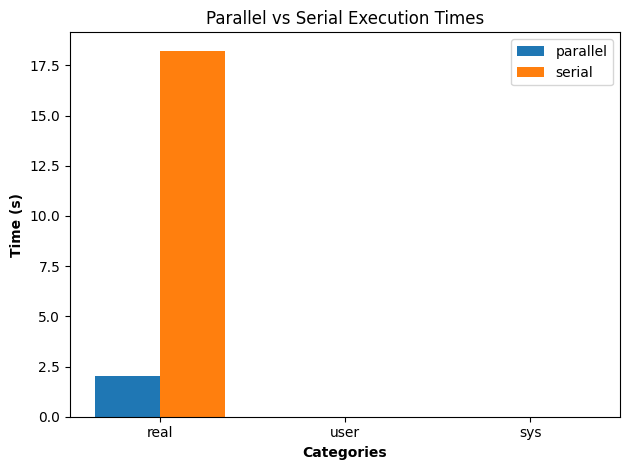
\includegraphics[width=0.8\linewidth]{./ex2.png}
	\caption{pingを並行して実行する関数と直列に実行する関数の性能測定結果}
	\label{fig:ex-2}
\end{figure}

実行時間のほぼすべてがuser timeで占められているのは,pingコマンドを実行して外部のレスポンスを待っていることが大半だからである.
また,並行に実行した場合の方が直列に実行した場合よりも実行時間が短いことがわかる.

今回は9つのホスト名を指定してそれぞれの関数を実行したが,並列に実行した場合が直列に実行した場合より9倍速いわけではなかった.
並列実行した場合,最もレスポンスが返ってくるのに時間を要したホストへのpingコマンドの実行時間が全体の実行時間に大きく影響する.
このため,並列実行した場合の実行時間が直列実行した場合の1ホストあたりの実行時間よりも短いとは限らないと考えられる.

\section{課題3}
\label{sec:ex-3}

課題で与えられた,コマンドを実行し標準入力に与えられたデータと同じものをログファイルに控えるプログラムを\ref{code:ex-3}のように作成した.

\begin{lstlisting}[language={C}, caption={コマンドを実行し標準入力に与えられたデータと同じものをログファイルに控えるプログラム}, label={code:ex-3}]
#include <fcntl.h>
#include <stdio.h>
#include <stdlib.h>
#include <string.h>
#include <sys/wait.h>
#include <unistd.h>

int main(int argc, char *argv[]) {
  if (argc < 3) {
    fprintf(stderr, "Usage: %s logfile command [args...]\n", argv[0]);
    return 1;
  }

  char *logfile = argv[1];
  char *command = argv[2];
  char **args = &argv[3];

  int pipefd[2];
  if (pipe(pipefd) == -1) {
    perror("pipe");
    return 1;
  }

  pid_t pid = fork();

  if (pid == -1) {
    // フォーク失敗
    perror("fork");
    exit(1);
  } else if (pid == 0) {
    // 子プロセス
    close(pipefd[1]);
    dup2(pipefd[0], STDIN_FILENO);  // リダイレクトする
    close(pipefd[0]);
    execvp(command, args);
    perror("execvp");
    exit(1);
  } else {
    // 親プロセス
    close(pipefd[0]);
    int logfd = open(logfile, O_WRONLY | O_CREAT | O_TRUNC, 0644);
    if (logfd == -1) {
      perror("open");
      exit(1);
    }

    char buffer[1024];
    ssize_t bytes;
    while ((bytes = read(STDIN_FILENO, buffer, sizeof(buffer))) > 0) {
      if (write(pipefd[1], buffer, bytes) == -1) {
        perror("write to pipe");
        exit(1);
      }
      if (write(logfd, buffer, bytes) == -1) {
        perror("write to logfile");
        exit(1);
      }
    }

    if (bytes == -1) {
      perror("read");
    }

    close(pipefd[1]);  // Close write end of pipe
    close(logfd);      // Close logfile

    // Wait for child process to finish
    wait(NULL);
  }

  return 0;
}
\end{lstlisting}

このコードをコンパイルして,実験資料で示された\verb|./a.out stdin_log more -10 < /usr/include/X11/Xlib.h|のようなコマンドを実行した.

動作結果としては,moreコマンドで表示した内容をどこまで見るかによって,ログファイルに書き込まれる量も異なるというようになった.
このような結果になる理由として,\verb|pipe()|の動作の仕組みが関係していると推測した.

\verb|pipe()|は,親プロセスと子プロセス間でデータをやり取りするためのパイプを作成するシステムコールである.
子プロセスはパイプの出力を標準入力にリダイレクトし,親プロセスは標準入力から受け取った内容をパイプの入力とログファイルに書き込んでいる.
このため,\verb|more|コマンドで標準入力を読み込んだ分だけパイプに入力され,ログファイルに書き込まれるということになる.

実際に,\verb|more|コマンドで表示する行数を変えて実行した結果,すべての行を表示した場合はログファイルにもすべての行が書き込まれ,
元ファイルと\verb|diff|コマンドで比較しても同じであることが確認できた.一方で途中の行までしか表示しなかった場合はログファイルにも途中までの行しか書き込まれなかった.

このような結果から,\verb|UNIX|が提供しているパイプはそのとき必要な分だけ\verb|IO|アクセスを行うことで,高速にプログラムを動作させる工夫がなされていると考えられる.

% \bibliography{hoge} %hoge.bibから拡張子を外した名前
% \bibliographystyle{junsrt} %参考文献出力スタイル
% 使用する際は latex-workshop.latex.recipe.default を
% ptex2pdf (uplatex) → bibtex → ptex2pdf (uplatex) × 2
% に変更

\end{document}
